\documentclass[a4paper]{report}
\usepackage[utf8]{inputenc}
\usepackage[numbers]{natbib} % scientific references in the bibliography
\usepackage{hyperref}
\usepackage{graphicx}
%\usepackage{datetime}
\usepackage{color}
\usepackage{perpage} %the perpage package
\MakePerPage{footnote} %the perpage package command
%\usepackage{microtype}
%\usepackage{draftwatermark}
\usepackage{tikz}

%% Nicely format and linebreak URLs in the bibliography
%\usepackage{url}

%% Nicer formatting of figure captions.
%\usepackage[font=small,format=plain,labelfont=bf,up,textfont=it,up]{caption}

%\SetWatermarkScale{5}

%% Define a new 'leo' style for the package that will use a smaller font.
%\makeatletter
%\def\url@leostyle{%
%  \@ifundefined{selectfont}{\def\UrlFont{\sf}}{\def\UrlFont{\small\ttfamily}}}
%\makeatother
%% Now actually use the newly defined style.
%\urlstyle{leo}

%\newcommand{\hi}[1]{{\color{red}\tiny \em #1\/}\\}
\newcommand{\todo}[1]{\footnote{{\color{red} TODO: #1}}}

% ------------------------------------------------------------------------------
% Metadata
% ------------------------------------------------------------------------------
\title{Ontology Learning from Swedish Text}

\author{Jan Daniel Bothma}

% ------------------------------------------------------------------------------
% Document
% ------------------------------------------------------------------------------
\begin{document}

\maketitle

\begin{abstract}
\end{abstract}	

\tableofcontents

\chapter{Introduction}
%ONE-SENT Ontology learning learning tools significantly speed up the knowledge extraction part of the Knowledge Engineering process. I'm going to investigate ontology learning from Swedish text.
%%UU-CHAP Motivation for the Project
%%UU-CHAP Background to the problem or system
%%"I am going to look at the following things"

By encoding semantic information about the world in a form that can be processed by computers, computers can provide better support in many tasks.


\section{Semantic Web}

\section{Ontologies}

\section{Ontology Engineering}

\section{Ontology Learning}

The automatic or semi-automatic construction of ontologies from domain data is called Ontology Learning \cite{Cimiano06}. 
Ontology Learning (OL) can start with structured, semi-structured or unstructured data as input \cite{Cimiano2009OL}.
Structured data, such as databases, can be somewhat independent of language and its semantics are described by its schema or structure \todo{I think \cite{Cimiano2009OL} is sufficient but need to check}.
Most methods for ontology learning from semi-structured data such as wikis and unstructured data in the form of plain text depend on preprocessing techniques from the field of Natural Language Processing (NLP) to provide syntactic annotations like part of speech or syntactic dependencies.
OL methods are then applied to the annotated corpus, each method extracting one or more kind of ontology element.

Ontology learning software systems have been implemented that provide one or more algorithms for extracting concepts, relations and axioms from a text corpus.
Such systems are often integrated with dedicated NLP tools to provide the required preprocessing facilities.
Extracted elements are manually or automatically added to an ontology and can often be output in a standard ontology serialisation format like OWL\cite{OWLOverview2004}.

Ontology learning methods have varying degrees of language dependence. 
In the simplest case, an OL system can be applied to another natural language by replacing the language models in the NLP components with models trained on the other language. 
However, often the syntactic and semantic structure of languages vary enough to require modifications to OL methods or the process as a whole \cite{Voelkner2008Spanish}\todo{saying "often" probably means we need more than one example}.

\section{Problem}
%ONE-SENT Hoewever, there is no Ontology Learning System for learning ontologies from Swedish text.

There appears to be no ontology learning software system that has been applied to learn ontologies from Swedish text.
\todo{Hjelm's thesis\cite{Hjelm09Thesis} learnt a "prototypal" ontology from several languages including swedish.
We can learn a bit from it, but he used terms from an existing ontology, and we need to check if the relations they learnt are applicable.
Given this, this sentence might be too strong}
There are some efforts to extract semantic data from Swedish text for some specific applications and domains
\todo{maybe need to be clearer why these aren't directly suitable, domain independence etc}, but to our knowledge, these have not been combined to extract concepts and relations and induce axioms from Swedish domain text.
\todo{cite what we know about here to demonstrate we have actually done a bit of searching}

\section{Objective}

The objective of this thesis is thus to investigate the application of Ontology Learning methods to Swedish text for the construction of domain ontologies. \todo{When I've chosen the methods I'm focusing on I can probably add another line or two to be more specific and why}

\section{Research Questions}

To fulfill this objective, this report attempts to answer the following research questions:

\begin{enumerate}
  \item{What are the general requirements for ontology learning research and application?\todo{how we derived this question isn't clear from the introduction. Either this becomes a side effect part of the method, or we need to justify this "product" in the intro before the questions}}
  \item{How do common ontology learning methods need to be modified to extract ontologies from Swedish text?\todo{I think we said this was too broad and I need to replace it with a comparison between two methods when I choose them. Perhaps the idea was just to compare our work compared to some baseline?}}
  \item{How do these modified methods perform compared to \todo{some baseline??? evaluation}?}
\end{enumerate}

\section{Approach}
%ONE-SENT

This section needs to identify and show how we avoid possible sources of bias.

The basis of our method is how OL has been applied to other comparable languages like German with its compounding, and what's been learnt from the existing work on information extraction from Swedish.

The implementation should probably be based on the architecture proposed in \cite{Cimiano2009OL}

NLP tools for the common annotations are available and under further development, partly as a result of the BLARK for Swedish project.

The procedure is something like set up preprocessing, apply existing methods to swedish, evaluate, tweak for swedish, evaluate.

Ideally we can repeat an experiment for English and reproduce their results, to support the assertion that our implementation is ok.

I think I'll evaluate taxonomy extraction against the Eurovoc thesaurus since I can probably get hold of corpora for one or more of the topics they cover.

The implementation will probably be integrated with some OE system. Protege 4+ looks nice since it has decent, modern libraries and tools and plugin framework.

\section{Delimitations}

it'd be nice but I probably won't be able to ground my ontologies in any upper ontologies (ontology matching and ontological architecture). Maybe this is easy or critical and I can revise this entry.

There's a lot of research into using internet phenomena like croud sourced data and stuff. We're focusing in extracting information from any Swedish text. This means we can produce results for domains that have very little or unrepresentative data online (but depends on finding some representative corpus). These approaches also have issues like access to the services and reliability of the data. For these reasons, we're not trying the web-sourced stuff specifically.

\section{Report Structure}

\chapter{Literature Review}
%%UU-CHAP Overview of relevant research and development that is used in specifying the problem and obtaining and evaluating appropriate solutions.
%%ONE-SENT Many methods for the subtasks have been developed for other languages, and some have already been applied to Swedish, but they have not been combined and evaluated as a pipeline. Furthermore, none of the existing OL systems are suitable to be extended to Swedish, nor support the necessary evaluation approaches.
%%UU-REQ Awareness of relevant prior research and development literature
%% -- comment on its relevance. In what way _is_ it relevant and in what way is it _not_ relevant.
%%UU-REQ critical appraisal of that literature as a basis for the formulation of project objectives and the conduct of the project.
%% -- quality of the literature affects its bearing on the project. Note on the quality of an evaluation keeping in mind whether a plain olde eval would have been suitable in the first place - what's the objective of the publication?

This chapter gives an overview of the theoretical background to this thesis. The relationships between Ontology Learning from Text and its surrounding disciplines are identified in Sec.\ref{sec:lit-rev:parents}, then work and issues relevant to this field and this thesis specifically are discussed in Sec.\ref{sec:lit-rev:immediate}.

\section{Parent disciplines}
\label{sec:lit-rev:parents}

This section identifies the relationships between Ontology Learning from Text, and the surrounding disciplines. At a high level, Knowledge Management and the Semantic Web form the basis of applications that are supported by semantics encoded in a manner that allows automated reasoning. Ontology Learning is related with Knowledge Acquisition and Representation as a specific form of these processes, and the relation between Machine Reading and Ontology Learning is covered briefly. Some of the parts Ontology Learning plays in Ontology Engineering are identified, and finally the broader field of Ontology Learning is described, leading to a definition of Ontology Learning from Text.

\begin{figure}
  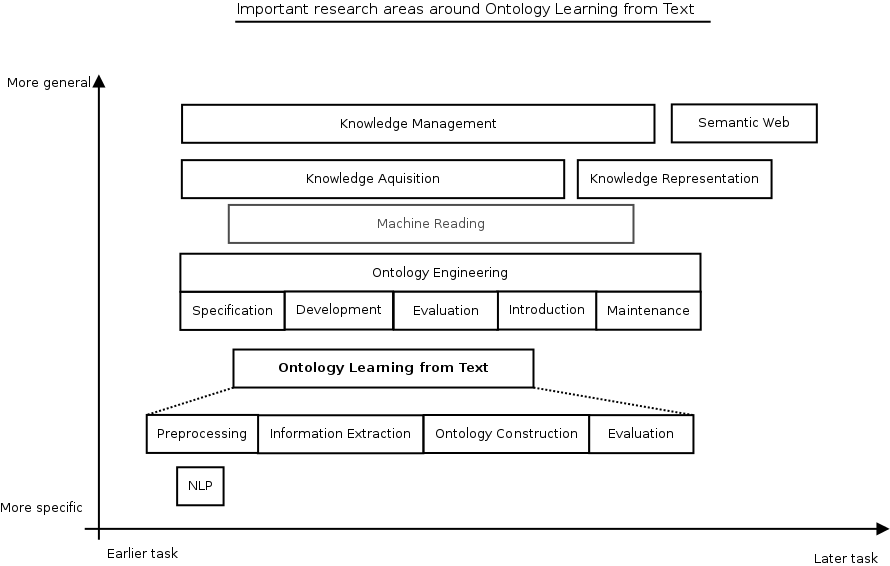
\includegraphics[width=\textwidth]{graphics/related-research-fields.png}
  \caption{Related research fields}
  \label{fig:related-research}
\end{figure}



\subsection{Knowledge Management}

Knowledge Management involves creation, storage, retrieval, transfer and application of the tacit and explicit knowledge pertaining to an organisation \citep{AlaviLeidner2001KM}.
Knowledge has been shown to be a significant asset in organisations, and information technology can help making such knowledge available to areas where the knowledge is not transferred easily \citep{AlaviLeidner2001KM}.

An example of using information technology to collect, store and apply valuable organisational knowledge is the \emph{semantically enabled} IURISERVICE iFAQ database of legal questions and answers given by experienced Spanish judges aims to support inexperienced judges in answering legal questions\cite{IURISERVICEPerformance2007}.
Important terms in the questions and answers are associated with their synonyms and the domain of law that they apply to.
When a question is entered to search for related question-answer pairs, the semantic information is used to improve the results over a plain text search, even when considering different forms of the words in the query.
The query is expanded to include exact matches, morphological variations\footnote{In the linguistic sense, such as \emph{car} to \emph{cars} for plurality}, and synonyms.
The similarity of the result questions to the query question is then calculated, considering the similarity of concepts and the grammatical structure of the questions, to provide the most-similar results to the user.
The semantic information is further used to provide suggestions of relevant legal cases whose decisions might have an impact on the issue at hand.

\subsection{Semantic Web}

By making semantically annotated information available over the internet, many resources can be combined to support complex tasks involving many parties.
The Semantic Web\footnote{http://www.w3.org/2001/sw/} is the manifestation of this.
In a hypothetical example, Tim Berners-Lee et al. \footnote{Tim Berners-Lee, James Hendler and Ora Lassila. The Semantic Web. \emph{Scientific American}, 284(August), p.3863170-3863170 2001} describe a scenario where a brother and a sister try to book medical appointments for their mother with a nearby treatment centre available to their mother's health insurance policy, on dates that they can alternate driving their mother.
Information about their availability, the clinics (including treatments they offer and their schedules) and the insurance policy must be available to the computers involved in proposing a solution.
Furthermore, the meaning of this information, and how it relates to the other information involved in the computation, must be available.
For example, the computer must be able to distinguish between the treatment centre's postal address and their visiting address.
This information is encoded in ontologies and mappings between semantic entities in standardised formats such as OWL\cite{OWLOverview2004} to support this interoperability.

The masses of information available as plain text is not directly usable in the semantic web. Knowledge must be encoded in machine-readable forms compatible with the Semantic Web. That knowledge can come from a variety of sources, and the process of gathering knowledge for storage and application in semantically-enabled systems is known as Knowledge Acquisition.

\subsection{Knowledge Acquisition}

Knowledge Acquisition in the context of information technology is the elicitation and interpretation of knowledge about a particular domain for use in knowledge-based systems \citep{anjewierden1987KATools}. This corresponds to the acquisition part of Knowledge Management and is a precursor to Knowledge Representation. 

\subsection{Knowledge Representation}


\subsection{Ontologies}
\label{sec:lit-rev:ontologies}

A commonly-cited definition of ontologies in the field of knowledge engineering is as \emph{``a formal, explicit specification of a shared conceptualization''} \cite{StuderEtAl1998KEPM}.
Here, a \emph{conceptualization} is the objects, concepts and relations between them, in an abstract view of the world intended for a particular purpose.
The conceptualization should be \emph{shared} within the context of its application.
The objective with this explicit specification is to allow computer agents to operate on this view of the world or for its integration in human-operated software.

Ontologies that represent a particular domain are known as \emph{Domain Ontologies}.
One way to support integration of several domain ontologies is by defining elements common to many domains in an \emph{upper ontology}\cite{SemanticIntegration2004Noy}.

\subsection{Ontology Engineering}

The discipline of specifying, developing, introducing and maintaining ontologies for some application is known as \emph{Ontology Engineering} (OE)\cite{HOO2009OntEngMeth}.
Along with broader considerations of OE such as the intended users and software engineering issues, the domain expert(s) and ontology engineer must gather relevant domain knowledge (Knowledge Acquisition) and encode it in a computer-readable form (Knowledge Representation)\cite{OntMethOverv1999}.
This is challenging and repetitive and is known as the Knowledge Acquisition Bottleneck\cite{OLforSemWeb2001}.
As an example, a "tasks and skills" ontology in the case study in \cite{HOO2009OntEngMeth} consisted of about 700 concepts after refinement. 
Automating as much as possible of the knowledge acquisition and representation can reduce the effort for domain experts and ontology engineers when developing and maintaining ontologies\todo{need to back this up}.

\subsection{Ontology Learning}

\subsection{Ontology Learning from Text}

This section defines Ontology Learning from text and discusses important work in this field. More detail of the tasks and methods of Ontology Learning from Text is covered in Sec.\ref{sec:lit-rev:immediate}

Ontology Learning from Text is the process of building a formal ontology from a semi-structured or unstructured text corpus from a particular domain \citep[p.3-7]{Cimiano06}. The ontology is intended to model the concepts and the semantic relationships between the concepts in the domain. Ontologies are further described in Sec.\ref{sec:lit-rev:ontologies}. 


The typical tasks and their outputs are shown in Fig.\ref{fig:output-task-technique}. 

\begin{figure}
  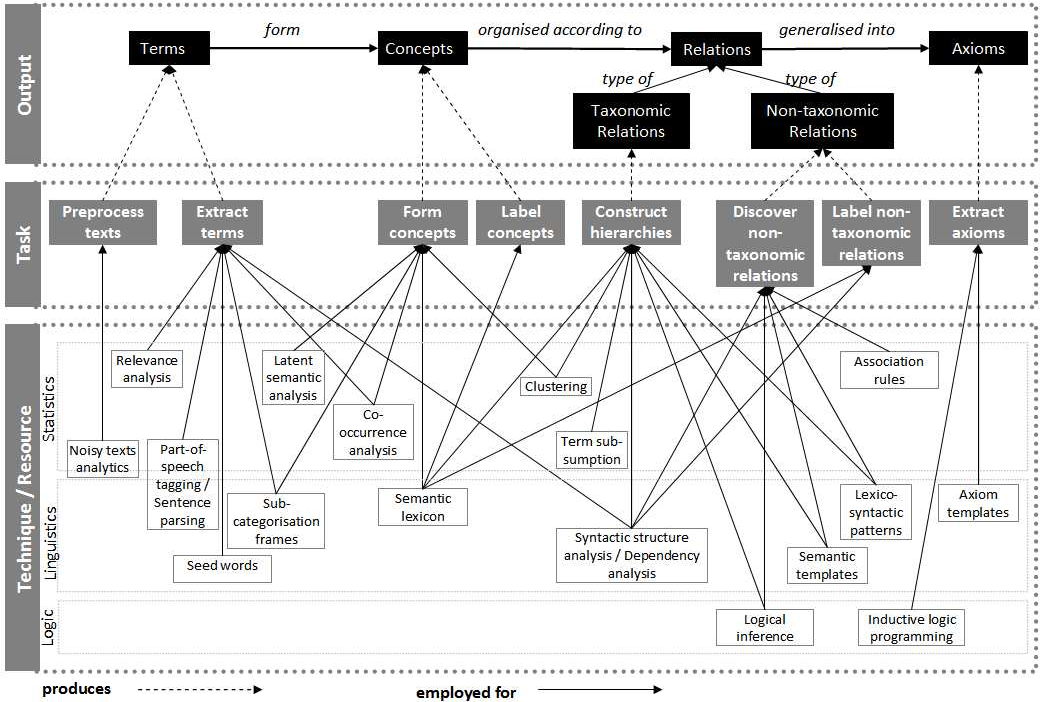
\includegraphics[width=\textwidth]{graphics/output-task-technique-WongLiuBennamoun.png}
  \caption{Tasks, techniques and outputs in ontology learning. \cite{Wong2009PhD}}
  \label{fig:output-task-technique}
\end{figure}


\subsection{Machine Reading}

Machine Reading is the automatic, unsupervised \emph{'understanding'} of text where understanding means formation of beliefs supporting some level of reasoning from a textual corpus \citep{EtzioniEtAll06MachineReading}. Machine Reading is distinguished from Information Retrieval where this is done in a in a highly supervised, manual manner - for example where patterns for extracting desired entities are hand-written or manually selected from an extracted list - striving instead for extracting arbitrary semantic relations without human supervision \citep{EtzioniEtAll06MachineReading}.

While Cimiano concluded that some level of supervision is necessary in Ontology Learning from Text \citep{Cimiano06}, recent work in Ontology Learning from Text such as OntoUSP\citep{Poon2010OntoUSP} and OntoCMaps \citep{Zouaq11OntoCmaps} shows progress towards learning arbitrary relations with high accuracy and recall in an unsupervised manner, which is much closer to machine reading than earlier work in the field.


\section{Immediate discipline}
\label{sec:lit-rev:immediate}

\begin{figure}
  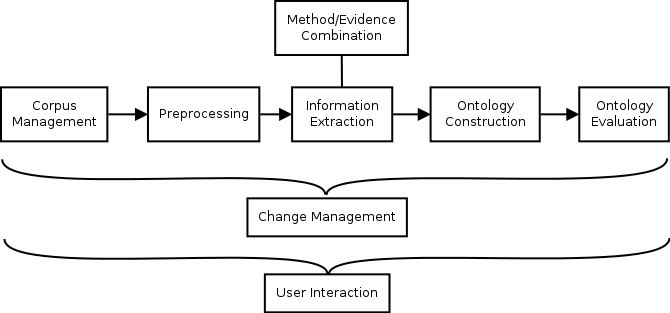
\includegraphics[width=\textwidth]{graphics/ontology-learning-system-issues.png}
  \caption{Issues for Ontology Learning systems}
  \label{fig:related-research}
\end{figure}

\subsection{Ontology Learning Steps}

\subsection{Corpus Management}

\subsection{Preprocessing}

\subsection{Information Extraction}

\subsubsection{Method / Evidence Combination}

\subsection{Ontology Construction}

\subsection{Ontology Evaluation}

\subsection{Change Management}

\subsection{User Interaction}

\chapter{Methodology}
%UU-CHAP Methods and techniques required
%ONE-SENT By making X modifications to existing methods, we can improve on the baseline of Y.   We evaluate these methods in by Z. We might even evaluate our evaluation tools.
%%Philosophy of Approach - show you can pick out important ideas succinctly
%%Plan of Attack - show you approached the problem in a systematic way

%UU-CHAP Implementation and formulation of the solution chosen
%ONE-SENT We implement a system that allows easy selection or combination of methods and their results, and allow the evaluation of these methods individually, in combination, and in pipeline.
%%Description of the work - details, so that others can follow what you did
%%  -> reproducibility

\section{Justification for the paradigm and methodology}

\section{Research Procedures}

\subsection{Preprocessing Swedish text}

\subsection{Term Extraction}

\subsection{Concept Formation}

\subsection{Concept Hierarchy}

\subsection{Relation Extraction}

\subsection{Ontology Construction}



\chapter{Analysis of data}
%%UU-REQ Evidence that the student has made a critical evaluation of the significance of the project outcomes, limitations of the results
%ONE-SENT We achieved results comparable to what was done with language Q in R. We can extract concepts and relations from Swedish text with evaluation metric S result of T.
%UU-CHAP Data collection and analysis where relevant, or testing of the solution of product.
%% Critical analysis of the results - show you know its limitations

\chapter{Conclusion and implications}
%%UU-CHAP Conclusions reached and future enhancement or work that could be conducted to refine the system.
%%UU-REQ Strength of the conclusions reached, including the ability to provide a concise summary of the significance of the work and reflect on work practice and outcomes with the intent to improve performance in future projects.
% summarise introduction with detail from Solution and Evaluation

\chapter{Further Work}
%% show you know what’s missing


\clearpage
%\addcontentsline{toc}{chapter}{References}
%\renewcommand\bibname{References}

%\renewcommand{\refname}{}
%\chapter{References}
\bibliographystyle{unsrt}
\bibliography{report}

\end{document}
